\documentclass{article}
\usepackage{amsmath}
\usepackage{zed-csp, graphicx}
%%%%%%%%%%%%%%%%%%%%%%%%%%%%%%%%%%%%%%%%%%%%%%%%%%%%%%%%%%%%%%%%
%  6.826 (POCS Seminar) macro file for handouts and problem sets.
%
% You should save this file as handout.tex
%
% Your main LaTeX file should look like this:
%
%        \documentstyle[12pt]{article}
%
%        %%%%%%%%%%%%%%%%%%%%%%%%%%%%%%%%%%%%%%%%%%%%%%%%%%%%%%%%%%%%%%%%
%  6.826 (POCS Seminar) macro file for handouts and problem sets.
%
% You should save this file as handout.tex
%
% Your main LaTeX file should look like this:
%
%        \documentstyle[12pt]{article}
%
%        %%%%%%%%%%%%%%%%%%%%%%%%%%%%%%%%%%%%%%%%%%%%%%%%%%%%%%%%%%%%%%%%
%  6.826 (POCS Seminar) macro file for handouts and problem sets.
%
% You should save this file as handout.tex
%
% Your main LaTeX file should look like this:
%
%        \documentstyle[12pt]{article}
%
%        \input{handout}
%%%%%%%%%%%%%%%%%%%%%%%%%%%%%%%%%%%%%%%%%%%%%%%%%%%%%%%%%%%%%%%%

\oddsidemargin 0in
\evensidemargin 0in
\marginparwidth 40pt
\marginparsep 10pt
\topmargin 0pt
\headsep 0in
\headheight 0in
\textheight 8.5in
\textwidth 6in
\brokenpenalty=10000

% \handout{number}{date}{title}

\newcommand{\handout}[3]{


\begin{center}
\rule{\textwidth}{.0075in} \\
\rule[3mm]{\textwidth}{.0075in}\\

CMU 17-651\hfill Models of Software Systems\hfill Fall 2018\\[3ex]

{\Large\bf #3}\\[3ex]

Dario A Lencina-Talarico \hfill {\bf Handout #1} \hfill #2

\rule{\textwidth}{.0075in} \\
\rule[3mm]{\textwidth}{.0075in} \\
\end{center}

}

% \homework{number}{date}{title}{due-date}
\newcommand{\homework}[4]{

\begin{center}
\rule{\textwidth}{.0075in} \\
\rule[3mm]{\textwidth}{.0075in}\\

CMU 17-651\hfill Models of Software Systems\hfill Fall 2018\\[3ex]

{\Large\bf #3} \\[3ex]

Dario A Lencina Talarico \hfill  #1  \hfill Due: #2\\

\rule{\textwidth}{.0075in} \\
\rule[3mm]{\textwidth}{.0075in} \\
\end{center}

%\noindent
%{\bf Due date: #4}

}

% \solutionset{number}{date}{title}{due-date}
\newcommand{\solutionset}[4]{

\begin{center}
\rule{\textwidth}{.0075in} \\
\rule[3mm]{\textwidth}{.0075in}\\

CMU 17-651\hfill Models of Software Systems\hfill Fall 2016\\[3ex]

{\Large\bf #3} \\[3ex]

Garlan  \hfill  Solutions for Homework #1  \hfill  #2\\

\rule{\textwidth}{.0075in} \\
\rule[3mm]{\textwidth}{.0075in} \\
\end{center}

%\noindent
%{\bf Due date: #4}

}

% \problem{problem-number}
\newcommand{\problem}[1]{
\vspace{2ex}
\noindent
{\bf Problem #1.}

}

% \solution{solution-number}{points}
\newcommand{\solution}[2]{
\vspace{3ex}
\noindent
{\bf Problem #1}  (#2 points)

}

\newcommand{\cscomment}{
\vspace{1ex}
\noindent Comments: }

% \parts{part-alphabet}{points}
\newcommand{\parts}[2]{
\vspace{2ex}
\noindent
{\bf (#1)}  (#2 points)

}

% \problems{problems-number}{points}
\newcommand{\problems}[2]{
\vspace{3ex}
\noindent
{\bf Problem #1}  (#2 points)

}

\newenvironment{symbolfootnotes}{\def\thefootnote{\fnsymbol{footnote}}}{}

%%%%%%%%%%%%%%%%%%%%%%%%%%%%%%%%%%%%%%%%%%%%%%%%%%%%%%%%%%%%%%%%

\oddsidemargin 0in
\evensidemargin 0in
\marginparwidth 40pt
\marginparsep 10pt
\topmargin 0pt
\headsep 0in
\headheight 0in
\textheight 8.5in
\textwidth 6in
\brokenpenalty=10000

% \handout{number}{date}{title}

\newcommand{\handout}[3]{


\begin{center}
\rule{\textwidth}{.0075in} \\
\rule[3mm]{\textwidth}{.0075in}\\

CMU 17-651\hfill Models of Software Systems\hfill Fall 2018\\[3ex]

{\Large\bf #3}\\[3ex]

Dario A Lencina-Talarico \hfill {\bf Handout #1} \hfill #2

\rule{\textwidth}{.0075in} \\
\rule[3mm]{\textwidth}{.0075in} \\
\end{center}

}

% \homework{number}{date}{title}{due-date}
\newcommand{\homework}[4]{

\begin{center}
\rule{\textwidth}{.0075in} \\
\rule[3mm]{\textwidth}{.0075in}\\

CMU 17-651\hfill Models of Software Systems\hfill Fall 2018\\[3ex]

{\Large\bf #3} \\[3ex]

Dario A Lencina Talarico \hfill  #1  \hfill Due: #2\\

\rule{\textwidth}{.0075in} \\
\rule[3mm]{\textwidth}{.0075in} \\
\end{center}

%\noindent
%{\bf Due date: #4}

}

% \solutionset{number}{date}{title}{due-date}
\newcommand{\solutionset}[4]{

\begin{center}
\rule{\textwidth}{.0075in} \\
\rule[3mm]{\textwidth}{.0075in}\\

CMU 17-651\hfill Models of Software Systems\hfill Fall 2016\\[3ex]

{\Large\bf #3} \\[3ex]

Garlan  \hfill  Solutions for Homework #1  \hfill  #2\\

\rule{\textwidth}{.0075in} \\
\rule[3mm]{\textwidth}{.0075in} \\
\end{center}

%\noindent
%{\bf Due date: #4}

}

% \problem{problem-number}
\newcommand{\problem}[1]{
\vspace{2ex}
\noindent
{\bf Problem #1.}

}

% \solution{solution-number}{points}
\newcommand{\solution}[2]{
\vspace{3ex}
\noindent
{\bf Problem #1}  (#2 points)

}

\newcommand{\cscomment}{
\vspace{1ex}
\noindent Comments: }

% \parts{part-alphabet}{points}
\newcommand{\parts}[2]{
\vspace{2ex}
\noindent
{\bf (#1)}  (#2 points)

}

% \problems{problems-number}{points}
\newcommand{\problems}[2]{
\vspace{3ex}
\noindent
{\bf Problem #1}  (#2 points)

}

\newenvironment{symbolfootnotes}{\def\thefootnote{\fnsymbol{footnote}}}{}

%%%%%%%%%%%%%%%%%%%%%%%%%%%%%%%%%%%%%%%%%%%%%%%%%%%%%%%%%%%%%%%%

\oddsidemargin 0in
\evensidemargin 0in
\marginparwidth 40pt
\marginparsep 10pt
\topmargin 0pt
\headsep 0in
\headheight 0in
\textheight 8.5in
\textwidth 6in
\brokenpenalty=10000

% \handout{number}{date}{title}

\newcommand{\handout}[3]{


\begin{center}
\rule{\textwidth}{.0075in} \\
\rule[3mm]{\textwidth}{.0075in}\\

CMU 17-651\hfill Models of Software Systems\hfill Fall 2018\\[3ex]

{\Large\bf #3}\\[3ex]

Dario A Lencina-Talarico \hfill {\bf Handout #1} \hfill #2

\rule{\textwidth}{.0075in} \\
\rule[3mm]{\textwidth}{.0075in} \\
\end{center}

}

% \homework{number}{date}{title}{due-date}
\newcommand{\homework}[4]{

\begin{center}
\rule{\textwidth}{.0075in} \\
\rule[3mm]{\textwidth}{.0075in}\\

CMU 17-651\hfill Models of Software Systems\hfill Fall 2018\\[3ex]

{\Large\bf #3} \\[3ex]

Dario A Lencina Talarico \hfill  #1  \hfill Due: #2\\

\rule{\textwidth}{.0075in} \\
\rule[3mm]{\textwidth}{.0075in} \\
\end{center}

%\noindent
%{\bf Due date: #4}

}

% \solutionset{number}{date}{title}{due-date}
\newcommand{\solutionset}[4]{

\begin{center}
\rule{\textwidth}{.0075in} \\
\rule[3mm]{\textwidth}{.0075in}\\

CMU 17-651\hfill Models of Software Systems\hfill Fall 2016\\[3ex]

{\Large\bf #3} \\[3ex]

Garlan  \hfill  Solutions for Homework #1  \hfill  #2\\

\rule{\textwidth}{.0075in} \\
\rule[3mm]{\textwidth}{.0075in} \\
\end{center}

%\noindent
%{\bf Due date: #4}

}

% \problem{problem-number}
\newcommand{\problem}[1]{
\vspace{2ex}
\noindent
{\bf Problem #1.}

}

% \solution{solution-number}{points}
\newcommand{\solution}[2]{
\vspace{3ex}
\noindent
{\bf Problem #1}  (#2 points)

}

\newcommand{\cscomment}{
\vspace{1ex}
\noindent Comments: }

% \parts{part-alphabet}{points}
\newcommand{\parts}[2]{
\vspace{2ex}
\noindent
{\bf (#1)}  (#2 points)

}

% \problems{problems-number}{points}
\newcommand{\problems}[2]{
\vspace{3ex}
\noindent
{\bf Problem #1}  (#2 points)

}

\newenvironment{symbolfootnotes}{\def\thefootnote{\fnsymbol{footnote}}}{}


\begin{document}

\homework{}{05 November 2018}{Homework \#10: Concurrency}{}

\begin{enumerate}

\item Traces and Specifications:

\begin{enumerate}
\item Enumerate the traces for the following process \verb"P":
\begin{verbatim}
 P = (a -> a -> END | b -> a -> END).
\end{verbatim}
$traces == $
$ \{ \langle a, a \rangle, \langle b, a \rangle, \langle a \rangle, \langle b \rangle, \emptyset \} $ \\

\item Enumerate the traces for the following process \verb"P":
\begin{verbatim}
 P1 = (a -> a -> END).
 P2 = (a -> b -> END | a -> c -> END).
 ||P = (P1 || P2).
\end{verbatim}
$traces ==  \{ \langle a, b \rangle, \langle a,c \rangle, \langle a \rangle, \emptyset \} $ \\
\\
It is important to mention that P1 seems to always deadlock as it requires 2 $a$ actions to reach the $END$ but P2 can only go through 1 a per run. \\
\end{enumerate}

\item More Concurrency:

Consider the two processes \texttt{STUDENT} and \texttt{TEACHER}, where
\begin{align*}
    \alpha\ \mathtt{STUDENT} &= \{\mathtt{do\_hw}, \mathtt{hand\_in}, \mathtt{pass}, \mathtt{fail}, \mathtt{cheer}, \mathtt{curse}\} \\
    \alpha\ \mathtt{TEACHER} &= \{\mathtt{hand\_in}, \mathtt{grade}, \mathtt{pass}, \mathtt{fail}, \mathtt{grumble}\}
\end{align*}
The student repeatedly does her homework, hands it in, and gets a pass or fail---cheering when she
passes and cursing when she fails. The teacher repeatedly collects the homework, grades it, and then assigns a pass or
fail grade---grumbling after any time that he has to give out a failing grade.

\begin{enumerate}
\item Write an FSP process that characterizes the student and show a diagram that indicates its
  behavior. \\
\begin{verbatim}
STUDENT = (do_hw -> hand_in -> STUDENT_SEND),

STUDENT_SEND = (pass -> cheer -> STUDENT | fail -> curse -> STUDENT).  
\end{verbatim}

\begin{center}
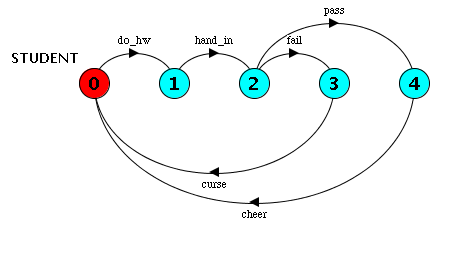
\includegraphics[width=3in]{STUDENT.png}
\end{center}

\item Write an FSP process that characterizes the teacher and show a diagram that indicates its
  behavior. \\

\begin{verbatim}
TEACHER = (hand_in->grade->TEACHER_GRADE_RESULT),

TEACHER_GRADE_RESULT = (pass -> TEACHER | fail -> grumble -> TEACHER).
\end{verbatim}

\begin{center}
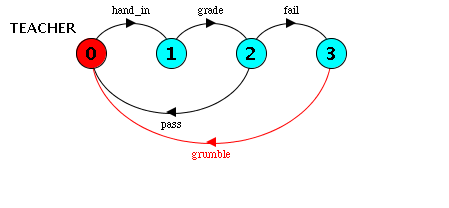
\includegraphics[width=3in]{TEACHER.png}
\end{center}  

\item Produce an LTS graph for \texttt{STUDENT || TEACHER}.

\begin{center}
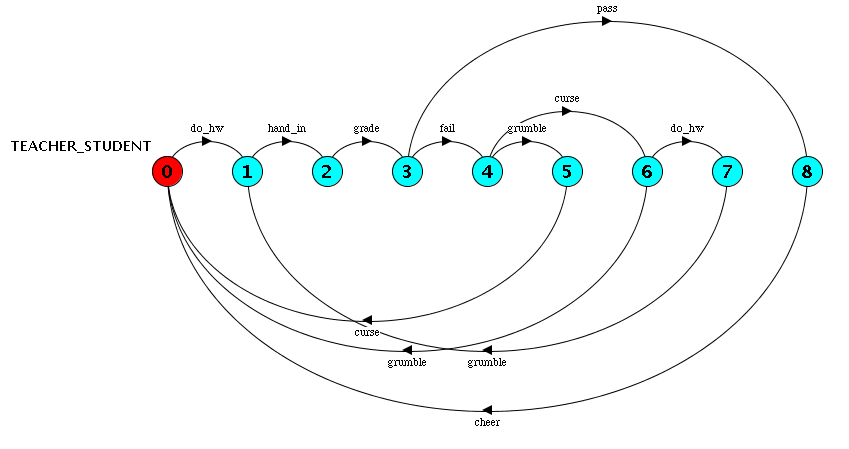
\includegraphics[width=5in]{TEACHER_STUDENT.png}
\end{center}

  
\item What happens to this process if we augment \texttt{STUDENT}'s alphabet with the \texttt{grumble} event and
have her grumble before doing her homework? Why does this occur? \\

$TEACHER\_STUDENT$ will deadlock because STUDENT will get stuck in grumble waiting for TEACHER to grumble, but TEACHER will get stuck waiting for the student to hand in the homework. 

\begin{center}
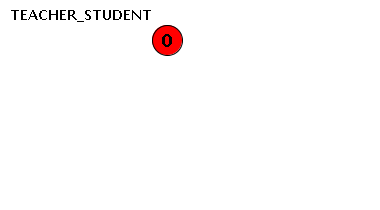
\includegraphics[width=3.5in]{DEADLOCK.png}
\end{center}
LTSA presents a nice warning message when executing the composition: 
\begin{center}
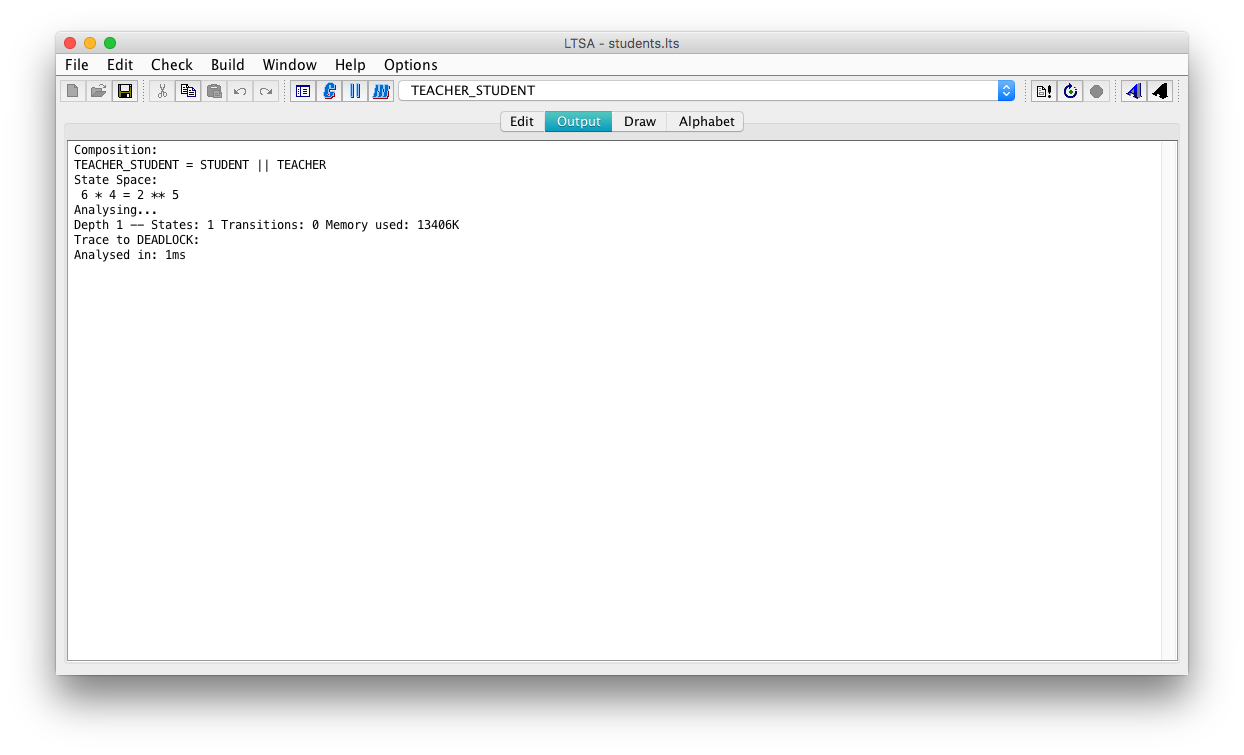
\includegraphics[width=5in]{DEADLOCK2.png}
\end{center}

\item If your answer to the previous question involves deadlock, list
two ways that you might change the definition to avoid this
unintended problem. ({\sc Note}: You may not change the order in which events happen. For example, do not move the student's \texttt{grumble} event after her \texttt{hand\_in} event. Preserve the intended behavior of the model.)
\end{enumerate}
Prefix grumbles with the name of the actor, teacher or student prevents the deadlock. \\
\begin{verbatim}
STUDENT = (student.grumble -> do_hw -> hand_in -> STUDENT_SEND),
       
STUDENT_SEND = (pass -> cheer -> STUDENT | fail -> curse -> STUDENT).

TEACHER = (hand_in->grade->TEACHER_GRADE_RESULT),

TEACHER_GRADE_RESULT = (pass -> TEACHER | fail -> teacher.grumble -> TEACHER).

||RESULT = (STUDENT || TEACHER).
\end{verbatim}
\begin{center}
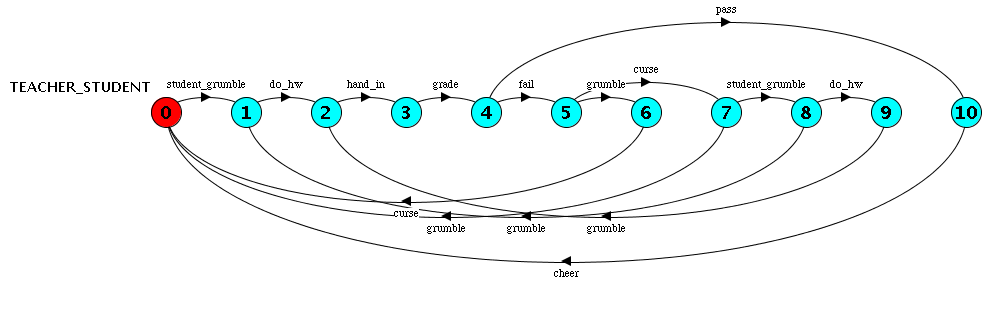
\includegraphics[width=6in]{student_grumble.png}
\end{center}

\item Exercises Based on MK06

Consider the model of the client--server system described in section~3.1.4 of MK06.
\begin{enumerate}
\item Extend the model of the client--server system so that more than one client can use the server. Your model should support an arbitrary number of clients (\texttt{N}). \\
\begin{verbatim}
const N = 2

CLIENT = (call->wait->continue->CLIENT).                                                      
                                                                                              
SERVER = (request->service->reply->SERVER).                                                   

||CLIENTS(M = 1) = (forall[i:1..M] s[i]:CLIENT). 

||CLIENT_SERVER = (CLIENTS(N) || SERVER)/{{s[1..N]}.call/request, {s[1..N]}.wait/reply}.
\end{verbatim}
Graph for CLIENTS N = 2 \\
\begin{center}
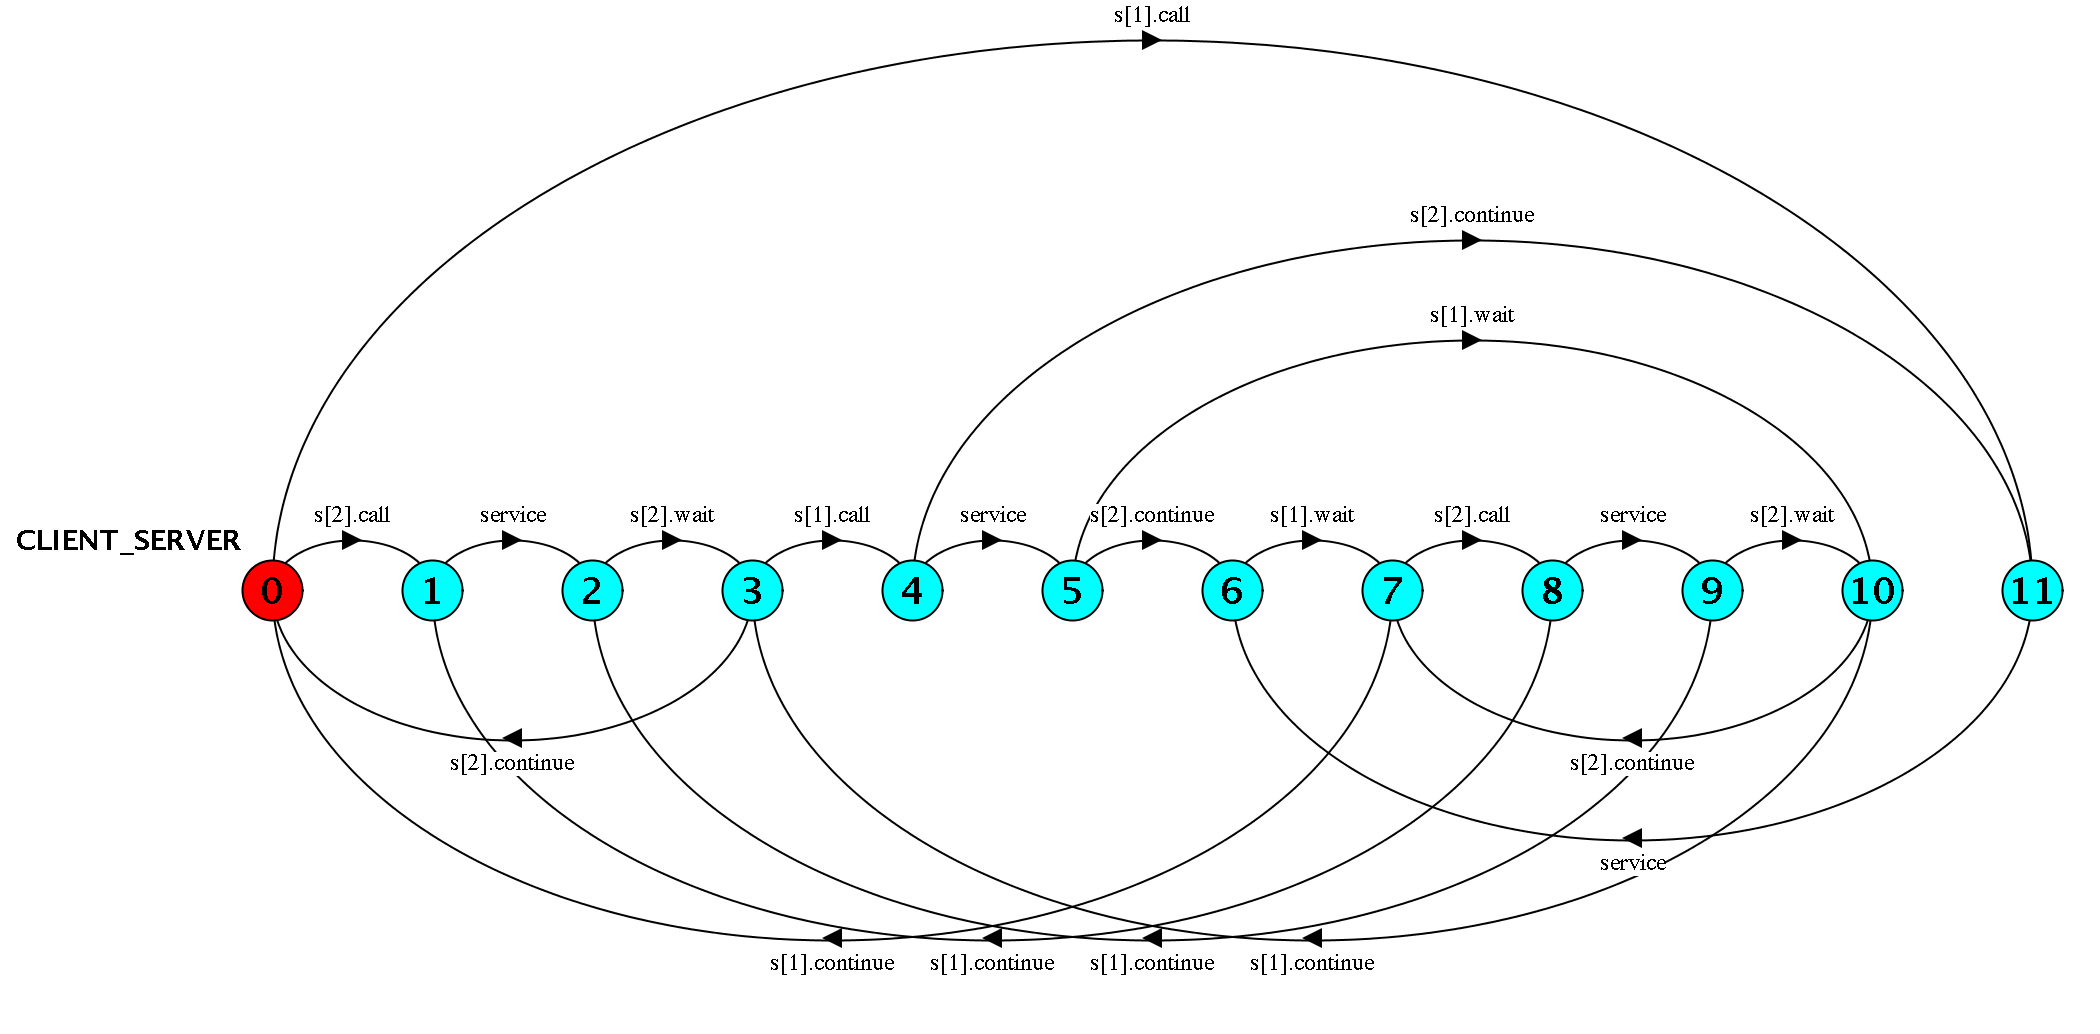
\includegraphics[width=6in]{CLIENT_SERVER_N2.png}
\end{center}

\item Modify your new model of the client--server system so that a client's call may terminate with a \texttt{timeout} action rather than a response from the server. (Do not modify the server process.) What condition results from this modification? \\
\\
My assumption is that if there's a timeout, the client will terminate as opposed to sending another request. \\
\\
The condition that results is a more realistic implementation of the client server model by incorporating a primitive error scenario. \\
  
\begin{verbatim}
const N = 1

CLIENT = (call->(wait->continue->CLIENT
                 | timeout->ERROR)).                                                    
                                                                                              
SERVER = (request->service->reply->SERVER).                                                   

||CLIENTS(M = 1) = (forall[i:1..M] s[i]:CLIENT). 

||CLIENT_SERVER = (CLIENTS(N) || SERVER)/{{s[1..N]}.call/request, {s[1..N]}.wait/reply}.
\end{verbatim}
\begin{center}
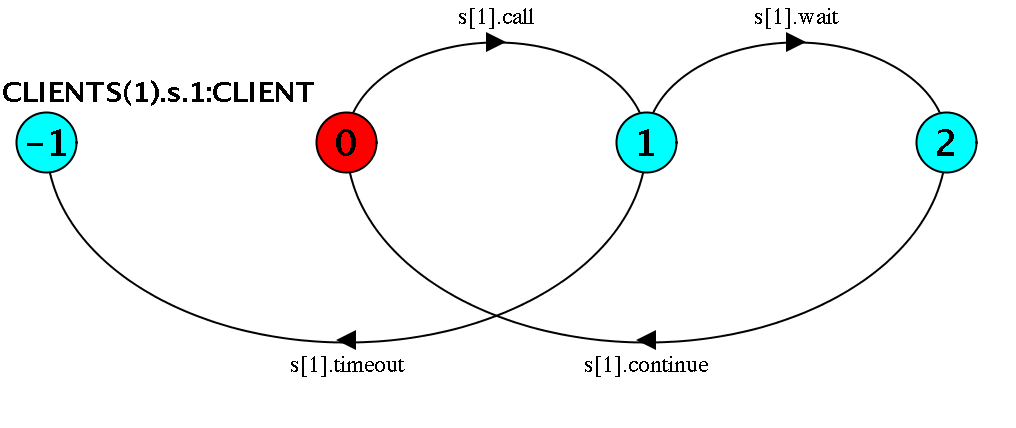
\includegraphics[width=3.5in]{CLIENT_WITH_ERROR_HANDLING.png}
\end{center}
\begin{center}
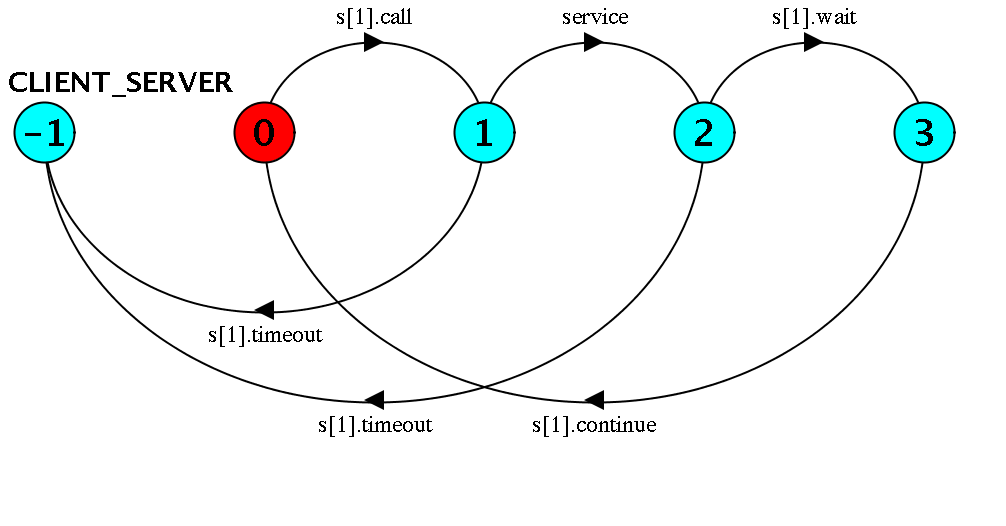
\includegraphics[width=3.5in]{CLIENT_WITH_ERROR_HANDLING_2.png}
\end{center}

\end{enumerate}
\end{enumerate}

\end{document}
